%%%%%%%%%%%%%%%%%%%%%%%%%%%%%%%%%%%%%%%%%%%%%%%%%%%%%%%%%%%%%%%
%                                                             %
%    Document class                                           %
%                                                             %
%%%%%%%%%%%%%%%%%%%%%%%%%%%%%%%%%%%%%%%%%%%%%%%%%%%%%%%%%%%%%%%

\documentclass[unicode,11pt,aspectratio=169]{beamer}

%%%%%%%%%%%%%%%%%%%%%%%%%%%%%%%%%%%%%%%%%%%%%%%%%%%%%%%%%%%%%%%
%                                                             %
%    Beamer theme for lecture in Meisei University            %
%                                                             %
%%%%%%%%%%%%%%%%%%%%%%%%%%%%%%%%%%%%%%%%%%%%%%%%%%%%%%%%%%%%%%%

\usepackage{packages/beamerthemeMeisei}

%%%%%%%%%%%%%%%%%%%%%%%%%%%%%%%%%%%%%%%%%%%%%%%%%%%%%%%%%%%%%%%
%                                                             %
%    Standard packages                                        %
%                                                             %
%%%%%%%%%%%%%%%%%%%%%%%%%%%%%%%%%%%%%%%%%%%%%%%%%%%%%%%%%%%%%%%

\usepackage{amsmath}
\usepackage{amsthm}
\usepackage{graphicx}
\usepackage{tikz}
\usepackage{tikz-3dplot}
\usetikzlibrary{cd}
\usepackage{clock}
\usepackage{bm}
\usepackage{lipsum}


%%%%%%%%%%%%%%%%%%%%%%%%%%%%%%%%%%%%%%%%%%%%%%%%%%%%%%%%%%%%%%%
%                                                             %
%    Additional packages                                      %
%                                                             %
%%%%%%%%%%%%%%%%%%%%%%%%%%%%%%%%%%%%%%%%%%%%%%%%%%%%%%%%%%%%%%%

\usepackage{packages/math}

%%%%%%%%%%%%%%%%%%%%%%%%%%%%%%%%%%%%%%%%%%%%%%%%%%%%%%%%%%%%%%%
%                                                             %
%    Body                                                     %
%                                                             %
%%%%%%%%%%%%%%%%%%%%%%%%%%%%%%%%%%%%%%%%%%%%%%%%%%%%%%%%%%%%%%%

\title{Title}
\subtitle{Subtitle}
\author{Name}
\institute{Institue}
\date{Date}

\begin{document}
\maketitle
% ----------------------------------------------------------- %
\section{First section}
% ----------------------------------------------------------- %
\begin{frame}{Frame title: sample text}
  
  \stc{
    \lipsum[1][1-3]
  }

  \stc{
    \lipsum[1][4-7] \\
    \lipsum[1][8-10]
  }

\end{frame}
% ----------------------------------------------------------- %
\begin{frame}{Frame title: column environment}
  \begin{columns}[c]

    \begin{column}{0.48\linewidth}

      \stc{
        \red{\lipsum[1][11-13]}
      }
      \stc{
        \lipsum[1][14-17]
      }

      \begin{center}
        \blue{{\Large \lipsum[1][18]\\ \lipsum[1][19]}}
      \end{center}

    \end{column}

    \begin{column}{0.48\linewidth}
      \begin{figure}[htbp]
        \centering
        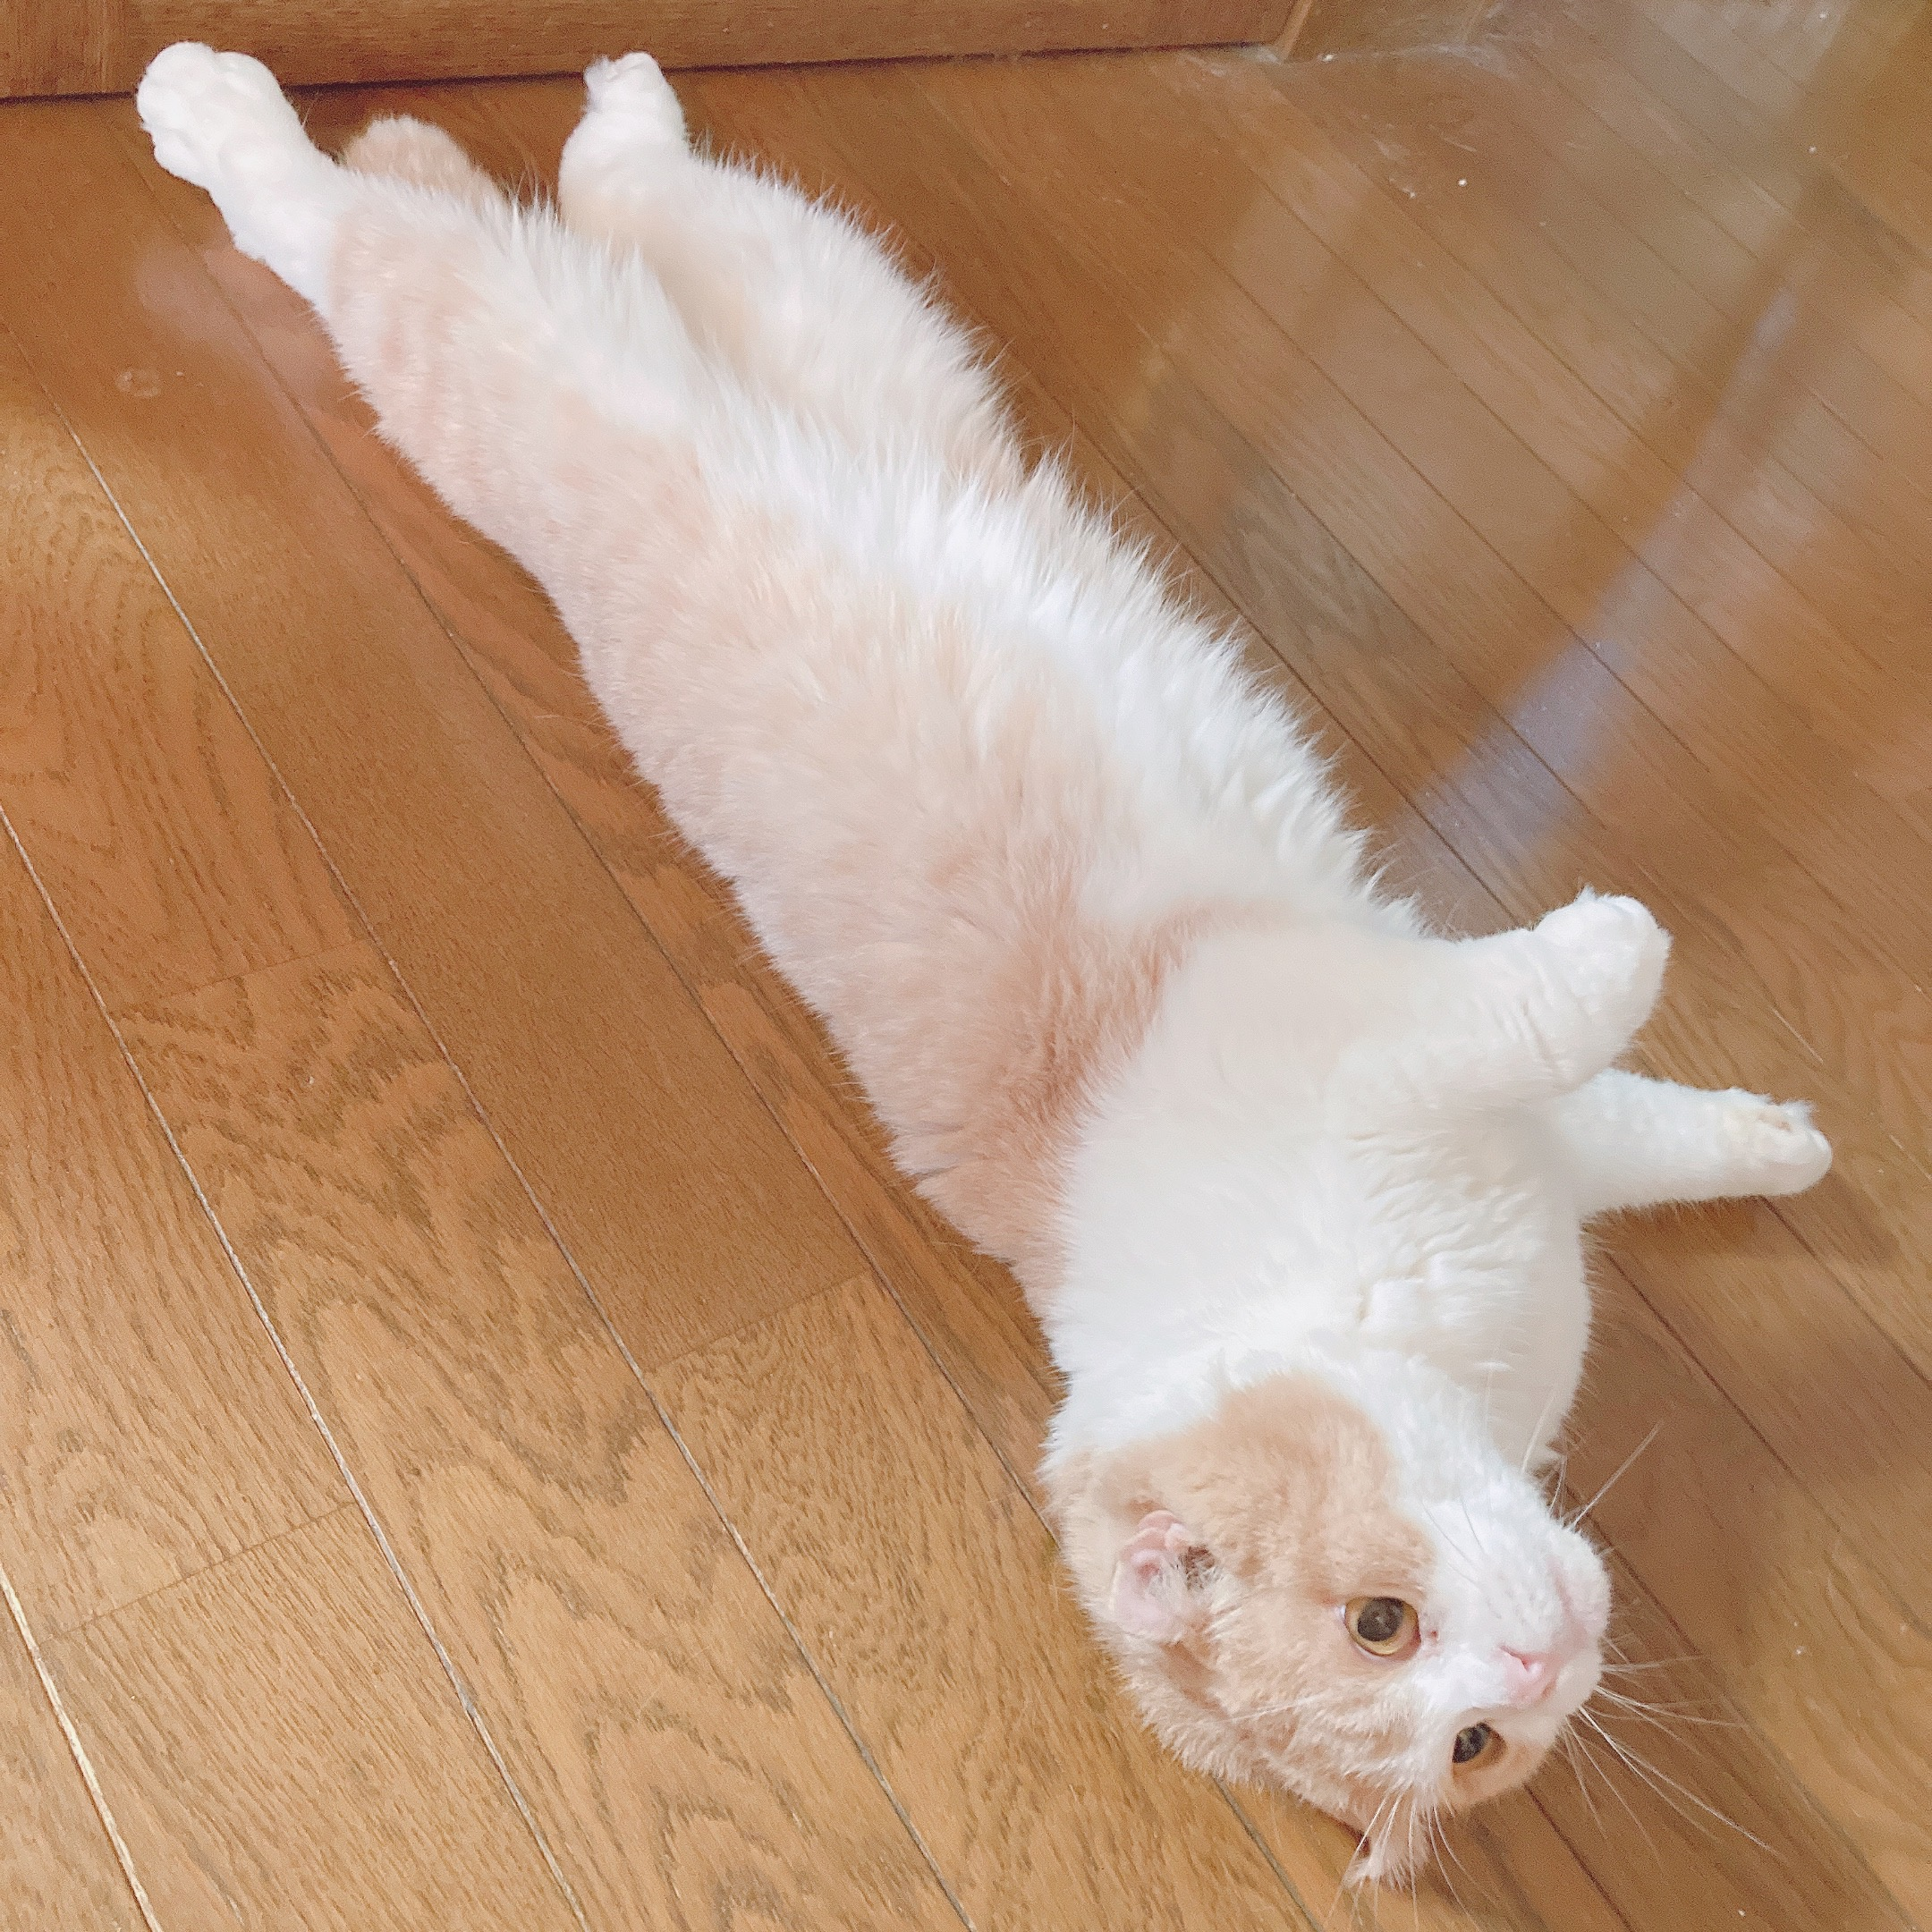
\includegraphics[height=6cm]{images/maron.png}
      \end{figure}
    \end{column}

  \end{columns}  
\end{frame}
% ----------------------------------------------------------- %
\section{Second section}
% ----------------------------------------------------------- %
\begin{frame}{Frame title: Theorem environment}

    \stc{
      \lipsum[2][1-3]
    }

  \begin{defi}[Optional text: Group homomorphism]
    Let $f: G\to H$ be a map between groups.
    We say that the map $f$ is \textit{group homomorphism}
    if it satisfies the following condition:
    \begin{align}
      \forall x, y\in G, \, f(xy)=f(x)f(y).
    \end{align}
  \end{defi}

\end{frame}
% ----------------------------------------------------------- %
\begin{frame}{Frame title: Theorem environment}
  \begin{thm}[Fundamental theorem of homomorphisms]
    For a group homomorphism $f: G\to H$, it holds that
    \begin{align}
      G/\Ker f\simeq \Im f, \, x\Ker f\mapsto f(x).
    \end{align}
  \end{thm}

  \vspace{-10pt}
  \begin{columns}[t]

    \begin{column}{0.48\textwidth}
      \stc{
        \lipsum[2][4-8]
      }
    \end{column}

    \begin{column}{0.48\textwidth}
      \begin{figure}[c]
        \centering
        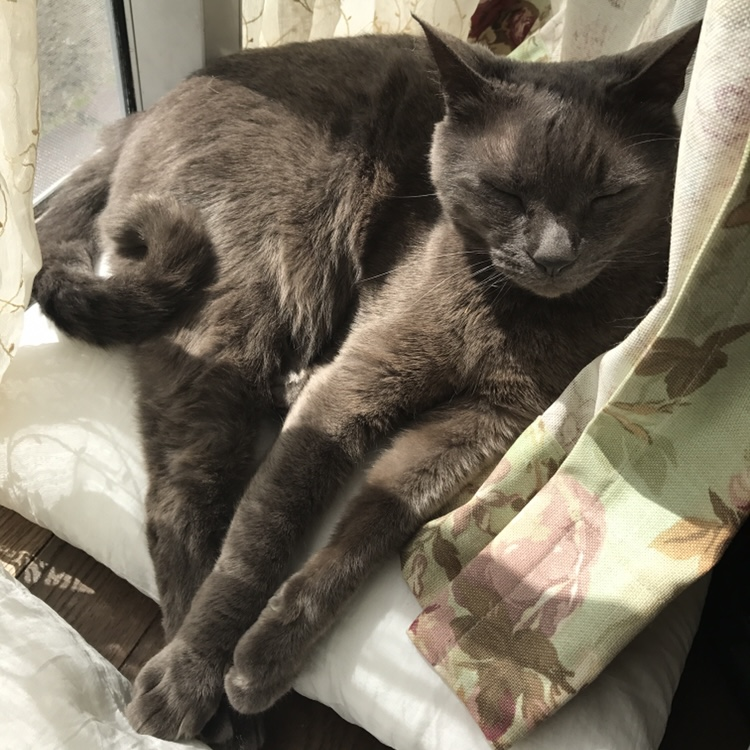
\includegraphics[height=3.5cm]{images/kuu.png}
        \vspace{-0.2cm}
        \caption{This is unrelated image.}
      \end{figure}
    \end{column}

  \end{columns}
\end{frame}
% ----------------------------------------------------------- %
\end{document}

